\section{eo\-Init\-Virus1bit$<$ Fit\-T $>$ Class Template Reference}
\label{classeo_init_virus1bit}\index{eoInitVirus1bit@{eoInitVirus1bit}}
Inits the virus with one bit to the left set to one.  


{\tt \#include $<$eo\-Init\-Virus.h$>$}

Inheritance diagram for eo\-Init\-Virus1bit$<$ Fit\-T $>$::\begin{figure}[H]
\begin{center}
\leavevmode
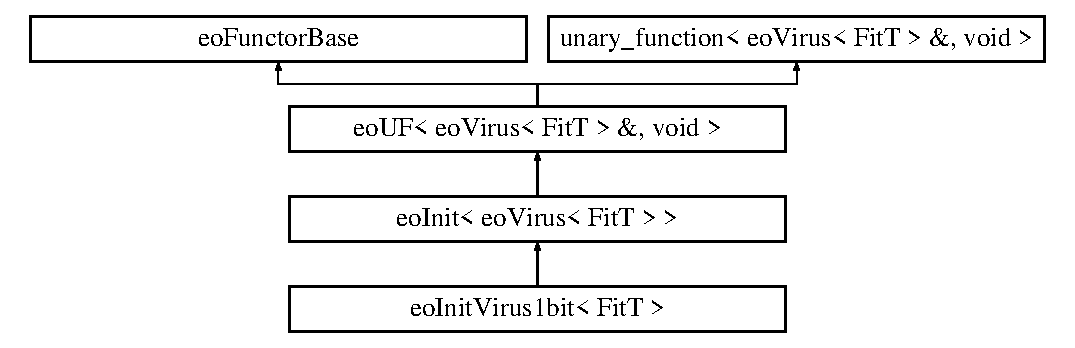
\includegraphics[height=4cm]{classeo_init_virus1bit}
\end{center}
\end{figure}
\subsection*{Public Member Functions}
\begin{CompactItemize}
\item 
{\bf eo\-Init\-Virus1bit} (unsigned \_\-combien, {\bf eo\-Rnd\-Generator}$<$ bool $>$ \&\_\-generator)\label{classeo_init_virus1bit_a0}

\item 
virtual void {\bf operator()} (eo\-Virus$<$ {\bf Fit\-T} $>$ \&chrom)\label{classeo_init_virus1bit_a1}

\begin{CompactList}\small\item\em The pure virtual function that needs to be implemented by the subclass. \item\end{CompactList}\end{CompactItemize}
\subsection*{Private Attributes}
\begin{CompactItemize}
\item 
unsigned {\bf combien}\label{classeo_init_virus1bit_r0}

\item 
{\bf eo\-STLF}$<$ bool $>$ {\bf generator}\label{classeo_init_virus1bit_r1}

\begin{CompactList}\small\item\em generic wrapper for eo\-Functor (s), to make them have the function-pointer style copy semantics \item\end{CompactList}\end{CompactItemize}


\subsection{Detailed Description}
\subsubsection*{template$<$class Fit\-T$>$ class eo\-Init\-Virus1bit$<$ Fit\-T $>$}

Inits the virus with one bit to the left set to one. 



Definition at line 66 of file eo\-Init\-Virus.h.

The documentation for this class was generated from the following file:\begin{CompactItemize}
\item 
eo\-Init\-Virus.h\end{CompactItemize}
